%!TEX root = ../thesis.tex
%*******************************************************************************
%*********************************** First Chapter *****************************
%*******************************************************************************

\chapter{Introduction}  %Title of the First Chapter

\ifpdf
    \graphicspath{{Chapter1/Figs/Raster/}{Chapter1/Figs/PDF/}{Chapter1/Figs/}}
\else
    \graphicspath{{Chapter1/Figs/Vector/}{Chapter1/Figs/}}
\fi


%********************************** %First Section  **************************************
\section{Motivation} %Section - 1.1 

Nowadays, there is a growing interest in exploiting the photos that users share on social networks such as Instagram or Twitter \cite{conf/bigdataconf/Tous16}, a part of the so-called user-generated content (UGC). On the one hand, users' photos can be analyzed to obtain knowledge about users behavior and opinions in general, or with respect to a certain products or brands. On the other hand, some users' photos can be of value themselves, as original and authentic content that can be used, upon users' permission, in different communication channels. However, discovering valuable images on social media streams is challenging. The amount of images to process is huge and, while they help, user defined tags are scarce and noisy. The most part of current solutions rely on costly manual curation tasks over random samples. This way many contents are not even processed, and many valuable photos go unnoticed. 

Some works, such as \cite{DBLP:journals/corr/ParkLK16}, \cite{conf/bigmm/TousTA15} or \cite{Denton:2015:UCH:2783258.2788576}, propose scene-based and object-based image recognition techniques to enrich the metadata originally present in social media images in order to facilitate their processing. Automatically tagging the incoming images with tags that describe their semantics (e.g. "beach", "car", etc.) enables more expressive filters and search conditions, minimizing manual curation. This way the time between the image publication and its detection and usage is minimized, the quality of the resulting photos increases (as more photos are analyzed and only the best ones go through manual curation) and the cost is reduced. 

Adoption of image recognition techniques in commercial UGC systems is currently very limited. In the best case they provide generic classifiers whose categories and original training data were not specific to UGC. Often these classifiers limit to the categories of the ImageNet Large Scale Visual Recognition Challenge (ILSVRC), but the vast majority of Instagram/Twitter photos are people-centric (selfies, food, clothes, etc.) while ILSVRC is more generic (fauna, flora, etc.). An important particularity of UGC is the huge amount of \textit{spam images}, i.e. images that, in the most usage scenarios, has no value neither as a knowledge carrier nor as a exploitable content. The incapacity of detecting the multiple types of spam images limits the usability and efficiency of existing solutions. Another difficulty of adopting image recognition techniques into UGC systems is the high computational cost of CNN-based image classifiers and object detectors. These systems need to process incoming streams of hundreds of images per second and a very volatile traffic. Any additional processing component need to be extremelly efficient and scalable. 

For all these reasons, the development of UGC systems that overcome the constraints imposed by manual curation (cost, qualty and delay time) requires the development of efficient and scalable image recogition pipelines, tailored for the particularities of UGC. 



%Figure \ref{fig:ui} shows the search interface of a UGC product commercialized by the company Adsmurai.

%\begin{figure}
%\begin{center}
%\centerline{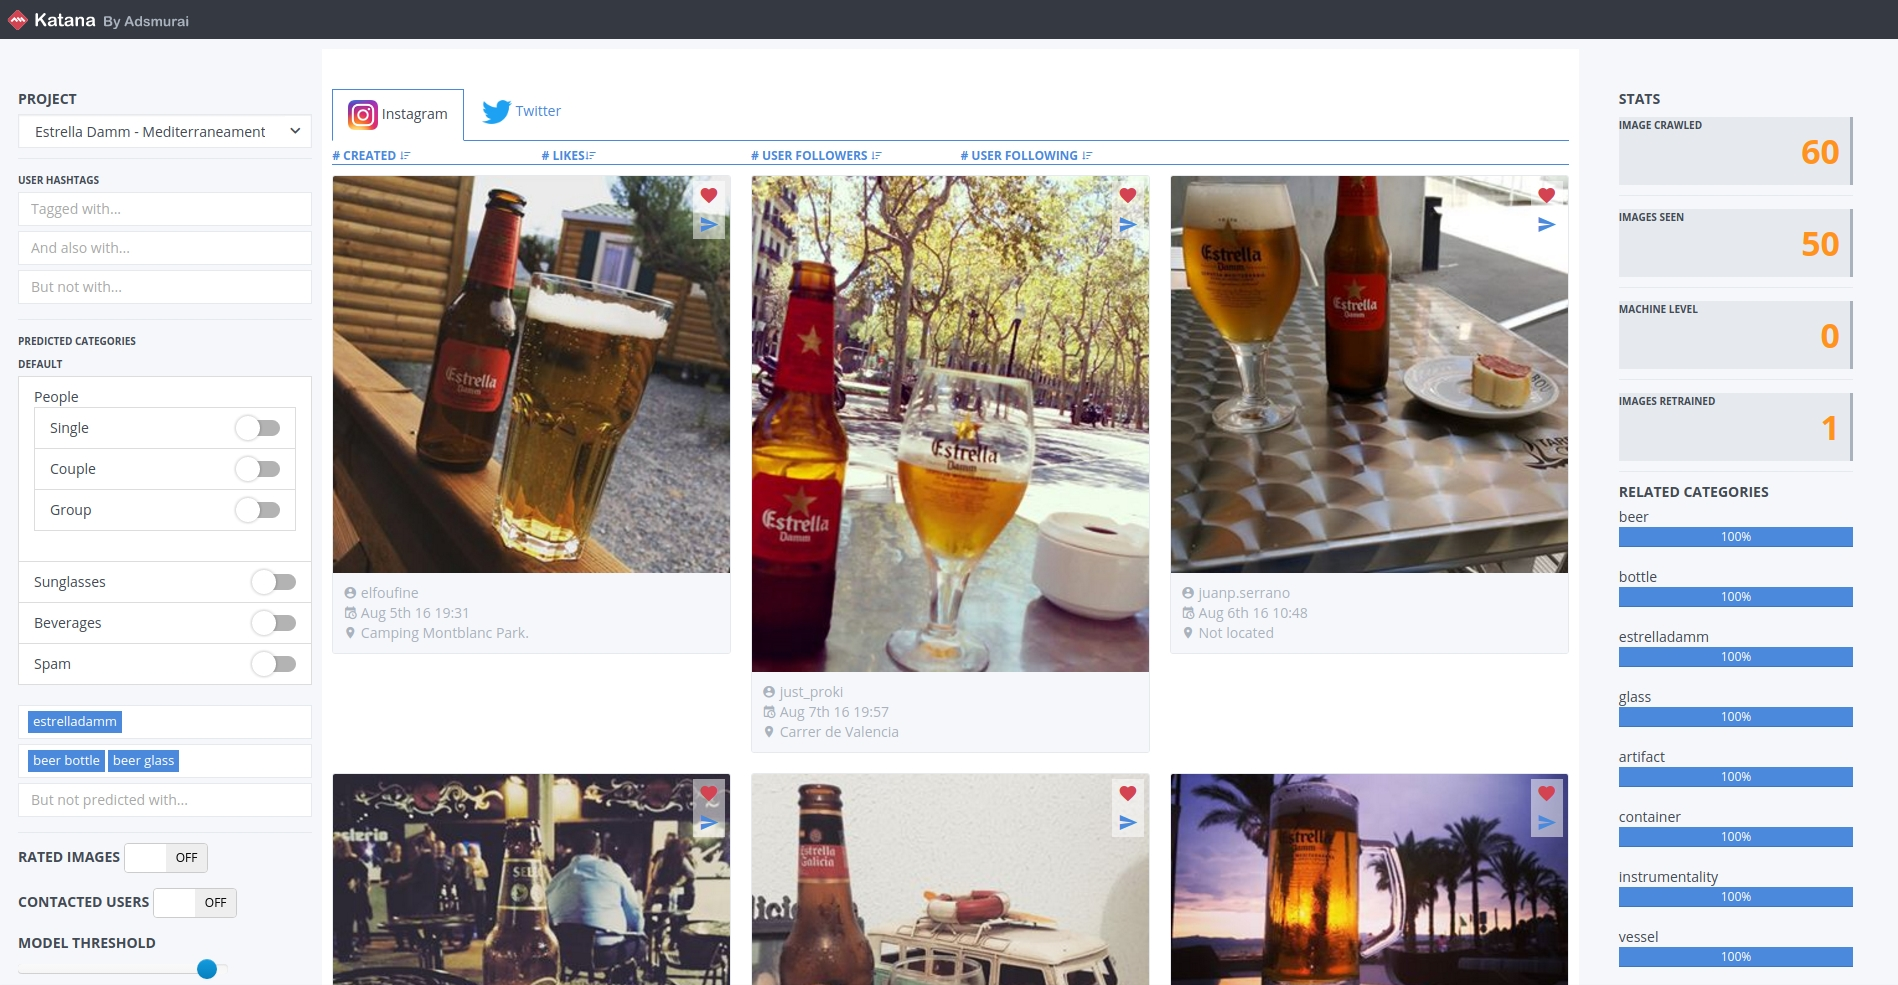
\includegraphics[width=3.0in]{Figs/ui1}}
%\caption{Screenshot of the user interface of the system, where users can navigate, search and select images from the database.} 
%\label{fig:ui}
%\end{center}
%\end{figure}





%********************************** %Second Section  *************************************
\section{Goals} %Section - 1.2


In this thesis, our general goal is to improve some techniques currently applied for automatically annotating photos posted by social media users. The generated annotations facilitate searching, filtering and analyzing user-generated content (UGC). We will apply scene-based and object-based image recognition techniques to extend the metadata originally present in the images with tags that describe their visual content. In order to reach state-of-the-art precission values we will employ CNNs. Performing these tasks in the UGC scenario implies some problems that are currently constraining their applicability to commercial systems. The specific goals of the project, that aim solving or mitigating some of these problems, are the following:

\begin{itemize} 
\item
Development of an efficient and scalable solution to enable complex image recogition pipelines for automatic UGC curation, where multiple CNN-based classifiers and object detectors can be chained in a graph fashion. The resulting solution must provide the necessary throughtput under reasonable cost assumptions, and must be able to scale. 
\item
Development of novel UGC-specific scene-based and object-based image recognition models, including but not limited to, a complete set of Instagram spam image detection models. 
\item
Development of a solution for the scalable training of on-demand custom classifiers and object detectors (e.g. company logos). Because of the particularities of these models, the resulting solution need to minimize training times and to be able to deal with small datasets. 
\end{itemize} 



\nomenclature[z-DKT]{DKT}{Draft Kiss Tumble}
\nomenclature[z-PPC]{PPC}{Particles per cell}